% nano-LMcache architecture figure — "Attention Is All You Need"-style block diagram.
% Compile:  pdflatex figure.tex   then   dvisvgm --pdf figure.pdf -o figure.svg
\def\pgfsysdriver{pgfsys-dvisvgm.def}   % native SVG specials -> no ghostscript needed
\documentclass[border=12pt]{standalone}
\usepackage{tikz}
\usetikzlibrary{arrows.meta, positioning, shapes.geometric, backgrounds, fit, calc}
\begin{document}
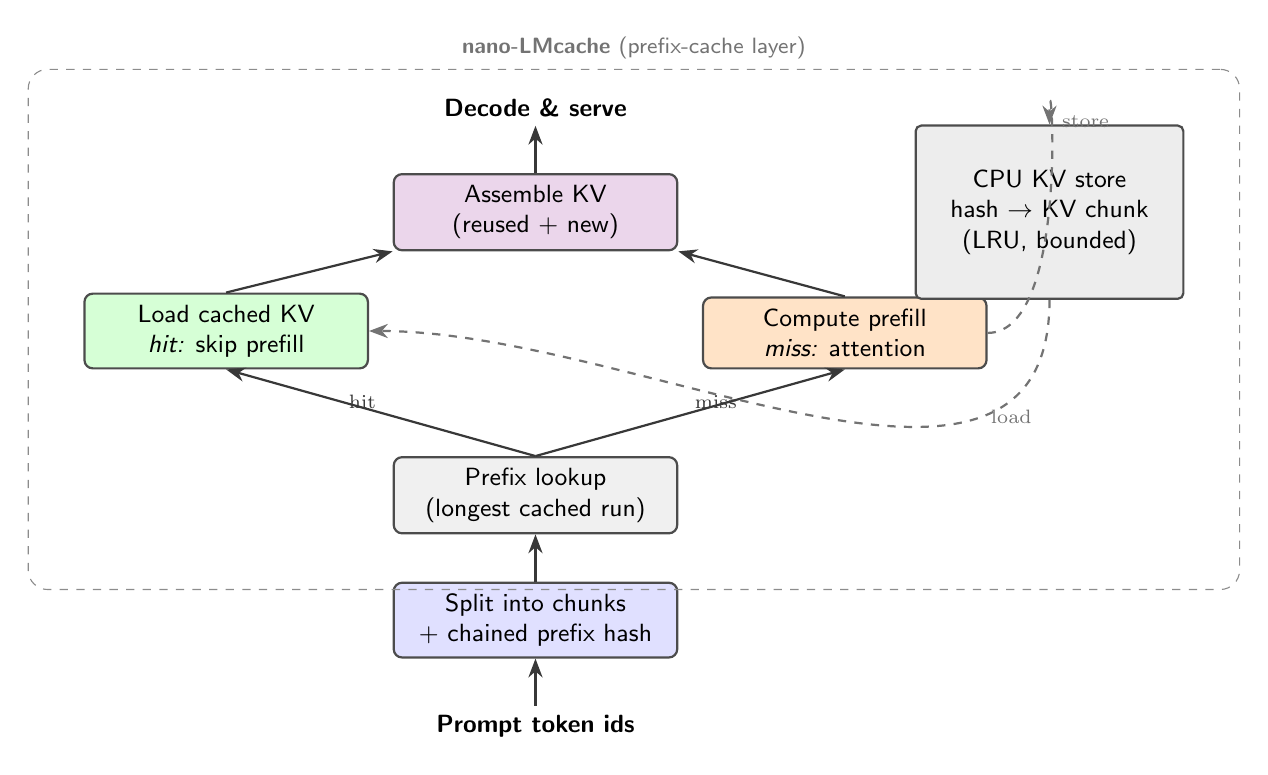
\begin{tikzpicture}[
  font=\sffamily\small, >=Stealth, node distance=6mm,
  block/.style={rounded corners=3pt, draw=black!70, thick, align=center,
                minimum height=9mm, minimum width=36mm, inner sep=4pt},
  hashb/.style={block, fill=blue!12},
  lookb/.style={block, fill=black!6},
  loadb/.style={block, fill=green!16},
  compb/.style={block, fill=orange!22},
  mrgb/.style={block, fill=violet!16},
  io/.style={align=center, font=\sffamily\small\bfseries},
  store/.style={rounded corners=2pt, draw=black!70, thick, fill=gray!14,
                align=center, minimum width=34mm, minimum height=22mm, inner sep=4pt},
  arr/.style={-{Stealth[length=2.4mm]}, thick, black!78},
  darr/.style={-{Stealth[length=2.4mm]}, thick, dashed, black!55},
]

% ---- main vertical flow (bottom -> top) ----
\node[io]    (tok)  at (0,0)                 {Prompt token ids};
\node[hashb, above=of tok]  (hash) {Split into chunks\\+ chained prefix hash};
\node[lookb, above=of hash] (look) {Prefix lookup\\(longest cached run)};
\node[loadb, above left=11mm and 3mm of look]  (load) {Load cached KV\\\emph{hit:} skip prefill};
\node[compb, above right=11mm and 3mm of look] (comp) {Compute prefill\\\emph{miss:} attention};
\node[mrgb, above=26mm of look] (asm) {Assemble KV\\(reused $+$ new)};
\node[io, above=of asm] (dec) {Decode \& serve};

\draw[arr] (tok)  -- (hash);
\draw[arr] (hash) -- (look);
\draw[arr] (look.north) -- (load.south) node[midway, above left=-1mm, font=\scriptsize]{hit};
\draw[arr] (look.north) -- (comp.south) node[midway, above right=-1mm, font=\scriptsize]{miss};
\draw[arr] (load.north) -- (asm.south west);
\draw[arr] (comp.north) -- (asm.south east);
\draw[arr] (asm)  -- (dec);

% ---- CPU KV store (the offload tier) on the right ----
\node[store, right=30mm of asm] (kv) {CPU KV store\\ hash $\to$ KV chunk\\ (LRU, bounded)};
\draw[darr] (comp.east) to[out=0, in=90]  node[pos=0.75, right, font=\scriptsize]{store} (kv.north);
\draw[darr] (kv.south)  to[out=-90, in=0] node[pos=0.25, right, font=\scriptsize]{load}  (load.east);

% ---- grouping box: the nano-LMcache layer (unfilled outline, drawn on top =
% no background layer needed, so no PostScript specials / no ghostscript) ----
\node[draw=black!45, dashed, rounded corners=7pt, fill=none,
      fit=(look)(load)(comp)(kv), inner sep=7mm,
      label={[black!55, font=\sffamily\footnotesize\bfseries]above:nano-LMcache \textmd{(prefix-cache layer)}}] {};

\end{tikzpicture}
\end{document}
